Nachdem im vorrigen Kapitel das episodiale Problem \textit{Jumping Dino} vorgestellt wurde, folgt nun die Darstellung eines kontinuierlichen Problems, dem \textit{AntGame}.
\par 
Inspiriert ist dieses Lernszenario durch die gleichnamige Semesteraufgabe in dem Wahlpflichtmodul \glqq Agentensysteme\grqq{} der Hochschule Bremerhaven. Zur Lösung jener Aufgabe implementierte der Autor dieser Arbeit bekannte Wegfindungsalgorithmen wie den A-Star und Explorationsmechaniken, die sich an der Tiefen- und Breitensuche orientierten. Die  Motivation für die Anwendung von Reinforcement Learning auf dasselbe Problem besteht darin, dass untersucht werden soll, ob RL-Algorithmen in der Lage sind, ähnliches Verhalten zu produzieren wie Algorithmen der klassischen Programmierung.
\par 
Konkret wird betrachtet, welche Schritte notwendig sind, um die ursprüngliche Aufgabenstellung zu einem RL-Problem umzuformulieren, damit u.a. die Markov-Eigenschaft erfüllt ist. Außerdem wird die Zielstrebigkeit untersucht und geschaut, ob der Agent implizit den A-Star Algorithmus lernen kann (Ausweichen von Hindernissen, direkter Weg zum Startpunkt).
\par 
Zunächst wird die originale Aufgabenstellung des Wahlpflichtkurses kurz vorgestellt. Anschließend werden Änderungen erläutert und die resultierende Umwelt präsentiert. Wie bei dem \textit{Jumping Dino} Lernszenario wird abschließend der Zustands- und Aktionsraum definiert und die Modellierung einer Belohnungsfunktion erläutert.

\subsubsection{Inspiration}
\begin{wrapfigure}{H}{0.5\textwidth}
    \begin{center}
    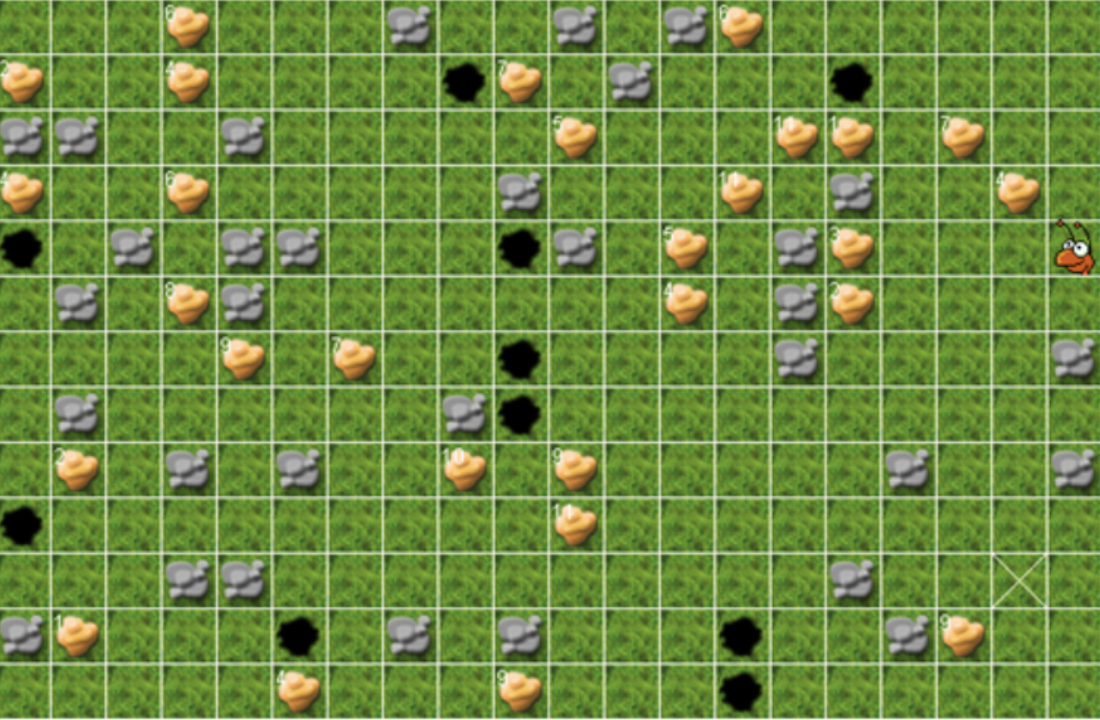
\includegraphics[width=200px]{images/rasterwelt.png}  \end{center}
    \caption{Rasterwelt}
    \label{fig:rasterwelt}
  \end{wrapfigure}
Die ursprüngliche Aufgabenstellung des Wahlpflichtkurses \glqq Agentensysteme\grqq{} ist stark an das Beispiel der \glqq Wumpus-Welt\grqq{} von \cite{wumpus} angelehnt (S.197-200). In einer Rasterwelt, siehe Abb. \ref{fig:rasterwelt}, befindet sich eine Ameise, die auf ihrem Nest spawnt. Ihr Ziel ist es, Futter zu suchen, es aufzusammeln und anschließend zu ihrem Nest zurückzulaufen, um es dort abzulegen. Dabei kann sie sich ausschließlich orthogonal bewegen, Hindernisse können ihren Weg blockieren und sie kann in Löcher fallen, die sie umbringen. Die Wahrnehmung der Ameise beschränkt sich auf die Erkenntnis auf welcher Art von Feld sie sich aktuell befindet sowie dem Futtergeruch bzw. Gestank orthogonaler Futterquellen respektive Löchern. 

\subsubsection{Problemstellung}
Es gibt zwei entscheidende Gründe, weshalb das ursprüngliche Problemszenario umformuliert werden muss. Zum einen kann das Feedback der Umgebung die Markov-Eigenschaft nicht erfüllen und zum anderen ist die Komplexität des Problems für die tabellarischen Lernmethoden deutlich zu hoch.
\par
Zunächst ist zu verdeutlichen, warum das originale Problem die Markov-Eigenschaft nicht erfüllen kann, die in Kapitel \ref{sec:MP} näher beleuchtet ist. Eine vereinfachte Variante der Informationen, die die Umwelt dem Agenten zukommen lässt, sieht wie folgt aus:
\begin{lstlisting}[language=json,firstnumber=1, label=lst:bar,caption=bar]
{
    "state": "ALIVE",
    "currentFood": 0,
    "totalFood": 0,
    "cell": {
        "row": 0,
        "col": 10,
        "type": "START",
        "food": 0,
        "smell": 0,
        "stench": 0
    }
}}
\end{lstlisting}
Bei einer solchen Zustandsmodellierung kommt es zu einem ähnlichen Problem wie bei dem, in Kapitel \ref{sec:MP} vorgestellten, Roboter-Beispiel. Angenommen, die Ameise befindet sich auf dem Feld mit den Koordinaten (0,10) und nimmt den Futtergeruch 1 wahr, dann kann die Ameise nicht logisch entscheiden, in welche Richtung sie sich bewegen muss. In einer Situation befindet sich das Futter auf dem nördlichen Nachbarsfeld, in einer anderen auf dem westlichen Nachbarsfeld. Für den Agenten sehen beide Situation identisch aus und er wird sich aufgrund des höhsten Aktions-Nutzens in beiden Fällen für dieselbe Aktion entscheiden.
\subsubsection{Zustandsmodellierung}

\subsubsection{Belohnungsfunktion}